\section{Additional Figures and Tables}\label{sec:appendix}

\begin{figure}[!h]
\centering
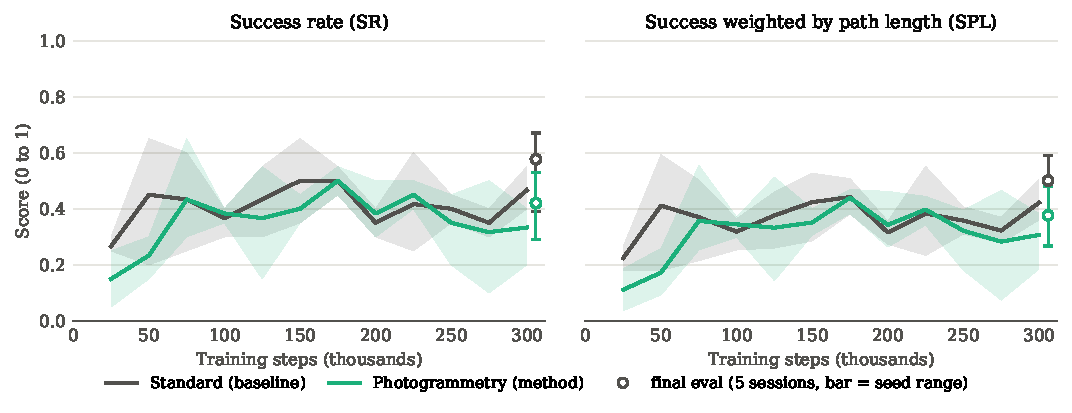
\includegraphics[width=\textwidth]{figures/training_curves}
\caption{Simulated SR (left) and SPL (right) during training, measured on the 20 routes every
25{,}000 steps (one session per point). Lines are the mean of the three seeds of each branch and
the shaded bands the range across seeds. Hollow markers at 300k are the final five-session
evaluations used in Table~\ref{tab:sim} (seed mean, bar showing the seed range). Single-session
evaluations of one seed jump by as much as 0.5 between neighbouring points, which is why the final
results use five sessions.}
\label{fig:training}
\end{figure}

\begin{figure}[!h]
\centering
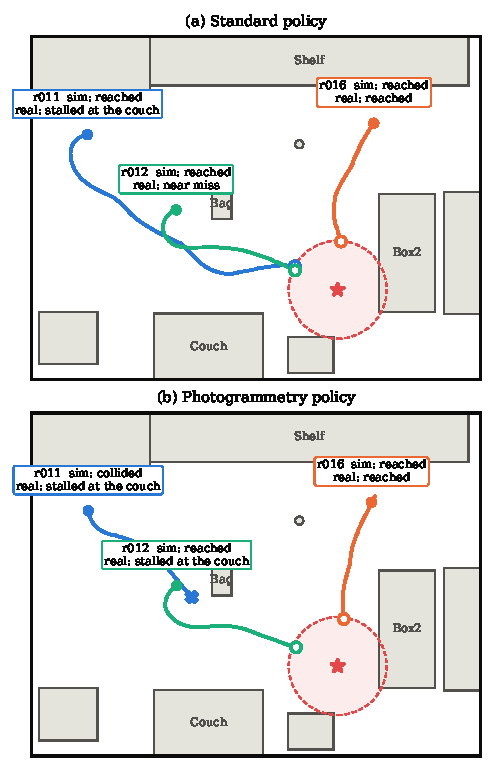
\includegraphics[width=0.42\textwidth]{figures/paths}
\caption{Simulated paths of the two deployed policies on three example routes (one rollout
each; filled dot: start, hollow circle: reached, cross: collision). The label gives the outcome
of the same route in simulation and on the real robot, whose path was not recorded.}
\label{fig:paths}
\end{figure}

\begin{figure}[!h]
\centering
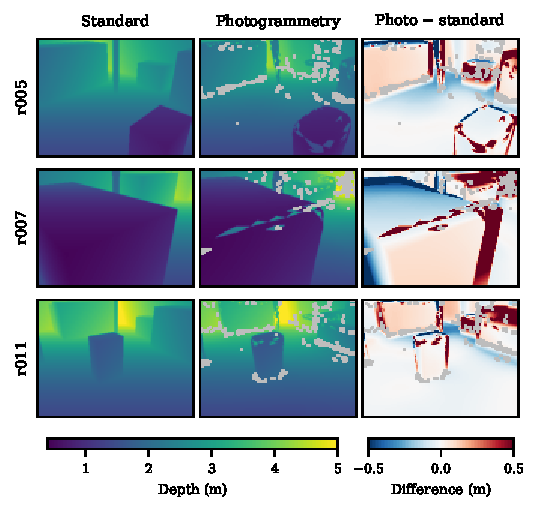
\includegraphics[width=0.42\textwidth]{figures/depth_compare}
\caption{Simulated depth images from identical poses in the two worlds: the head camera at the
start of three routes, turned to face the goal, with no robot in the scene. The right column is
photogrammetry minus standard depth. Grey pixels have no depth reading and are read by the policy
as far away; in the photogrammetry world they mostly come from small cracks in the scanned mesh.
The two worlds agree on the walls and floor, and differ mainly at the edges of objects, where the
scanned shapes replace the standard world's boxes.}
\label{fig:depth}
\end{figure}
